% Generated by scripts/txt2tex.py from chapters/chapter_03.txt. Edit the TXT, not this file.
\chapterquestion{מה נשאר מהשאלה על הבצק ברגע שהיא נכנסת אל תוך המכונה?}
\chapter{הרשת הנוירונית מבפנים}\label{ch:03}
\section{אין בצק בפנים}
השאלה של הקוראת כבר יצאה לדרכה. היא הקלידה "בצק", "תופח", "עכשיו", אבל ברגע שהמילים חוצות את גבול המסך הן מפסיקות להיות מילים. בתוך המערכת אין קמח, אין שיש ואין ערב מאוחר. יש מספרים. איך בדיוק טקסט הופך לרצף של מספרים נראה בפרק הבא; כאן נניח שההמרה כבר קרתה, ונרד אל היחידה הקטנה ביותר שמעבדת אותם: הנוירון המלאכותי (artificial neuron).
בפרק 1 דימינו את הפרמטרים של רשת לכפתורים במערבל קול. עכשיו נפרק את הלוח ונבדוק מה מחובר לכל כפתור.
\section{שקילה לפני החלטה}
דמיינו שאתם מתלבטים אם לצאת לטיול ערב. כמה שיקולים עולים בבת אחת: תחזית הגשם, העייפות, חבר שהציע להצטרף. לכל שיקול כובד משלו. תחזית סוערת דוחפת בתוקף נגד, ההזמנה מושכת בעדינות בעד. ויש גם נטייה כללית שקיימת עוד לפני כל שיקול: יש מי שיוצאים כמעט תמיד, ויש מי שנשארים בבית כמעט תמיד.
נוירון מלאכותי עושה משהו דומה, רק בלי לדעת על מה הוא מחליט. לפי רשימות הקורס CS231n של אוניברסיטת סטנפורד, כל נוירון מכפיל כל קלט במשקולת שלו, מחבר את המכפלות, מוסיף הטיה (bias) ומפעיל על התוצאה פונקציה לא-ליניארית \cite{S-ch03-01}. המשקולות (weights) הן עוצמות ההשפעה: הן קובעות כמה כל קלט "נחשב", ומה שחשוב יותר, הן נלמדות \cite{S-ch03-01}. משקולת חיובית גדולה מגבירה קלט, משקולת שלילית הופכת אותו לשיקול נגד, ומשקולת קרובה לאפס כמעט מתעלמת ממנו. ההטיה היא הנטייה הכללית: מספר קבוע שמזיז את התוצאה למעלה או למטה, בלי קשר למה שנכנס. אל תבלבלו אותה עם ההטיה מפרק 2, זו שמסתתרת בנתונים ופוגעת בהוגנות. כאן מדובר במספר אחד נוסף בחשבון, שבמקרה חולק איתה את השם, גם באנגלית.
זה מה שמסתתר מאחורי הלוח: כל משקולת וכל הטיה הן מספר אחד שאפשר לכוונן, והתפשטות לאחור היא האלגוריתם שמסמן לאיזה כיוון לשנות כל אחד מהם בזמן האימון \cite{S-ch01-05}.
\section{הנוסחה, סימן אחר סימן}
את מה שתואר במילים אפשר לכתוב בשורה אחת:
\begin{equation}
z = \sum_{i=1}^{n} w_i x_i + b
\end{equation}
x\_i: הקלט שמספרו i, אחד המספרים שנכנסים לנוירון. w\_i: המשקולת של אותו קלט. w\_i x\_i: המכפלה, כלומר כמה הקלט שוקל אחרי שהוכפל בחשיבות שלו. \textbackslash{}sum\_\{i=1\}\textasciicircum{}\{n\}: האות היוונית סיגמה מורה "חברו את כולם", מהקלט הראשון (i = 1) ועד האחרון. n: מספר הקלטים. b: ההטיה, שמתווספת לסכום פעם אחת. z: התוצאה, הסכום המשוקלל. מספר בודד.
ואז הצעד השני:
\begin{equation}
a = f(z)
\end{equation}
האות f מסמנת את פונקציית ההפעלה, ו-a הוא הפלט של הנוירון, המספר שימשיך הלאה. בחומרי הקורס של סטנפורד שני הצעדים כתובים כביטוי אחד, שבו הפונקציה עוטפת את הסכום \cite{S-ch03-01}. הספר מפריד ביניהם כדי שנוכל לעצור ולהתבונן בכל צעד לחוד.
\begin{labbox}{נוירון צעצוע בערב של הקוראת}
מספרים להמחשה בלבד. דמיינו נוירון עם שלושה קלטים שהגיעו מתוך השאלה על הבצק: $x_{1}$ = 0.9, $x_{2}$ = 0.2, $x_{3}$ = 0.5. המשקולות: $w_{1}$ = 1.5, $w_{2}$ = -2.0, $w_{3}$ = 0.8, וההטיה b = -0.5.
z = 1.5$\times$0.9 + (-2.0)$\times$0.2 + 0.8$\times$0.5 + (-0.5) = 1.35 --\ 0.4 + 0.4 --\ 0.5 = 0.85
נשתמש בפונקציית ReLU, שנכיר בהמשך הפרק: היא הופכת כל מספר שלילי לאפס ומשאירה מספר חיובי כמו שהוא. a = max(0, 0.85) = 0.85. הנוירון "דולק" ומעביר ערך הלאה.
עכשיו נשנה קלט אחד, $x_{2}$ = 0.9. הפעם z = 1.35 --\ 1.8 + 0.4 --\ 0.5 = -0.55, ולכן a = max(0, -0.55) = 0. הנוירון שותק.
ומה מייצג כל אחד מהמספרים האלה? שום דבר שאפשר לקרוא לו בשם. אף אחד מהם אינו "שמרים", ואף אחד אינו "סבלנות".
\end{labbox}
\section{ברז, לא מתג}
הסכום המשוקלל הוא חשבון ישר. הצעד השני מכניס לתוכו עיקום, ולכן מכנים אותו "אי-הליניאריות" של הנוירון \cite{S-ch03-01}.
פונקציה אחת כזאת היא הסיגמואיד (sigmoid), ואפשר לדמות אותה לשסתום שנפתח בהדרגה. היא דוחסת כל מספר אל הטווח שבין 0 ל-1, בנוסחה $\sigma$(z) = 1/(1 + e\textasciicircum{}(-z)) \cite{S-ch03-01}. אבל בקצוות העקומה משתטחת, מצב שנקרא רוויה (saturation), ושם כמעט נעלם השיפוע (gradient): האות שהתפשטות לאחור צריכה כדי לדעת לאיזה כיוון לשנות כל משקולת \cite{S-ch03-01}. ויש לה פגם נוסף: הפלט שלה אינו ממורכז סביב אפס \cite{S-ch03-01}. כל מה שהיא מוציאה חיובי, ולכן השכבה שאחריה מקבלת ממנה רק קלטים חיוביים.
כאן נכנסת לתמונה קרובת משפחה, הטנגנס ההיפרבולי (hyperbolic tangent, ובקיצור tanh). הנוסחה שלה נשענת על הסיגמואיד עצמה: tanh(z) = 2$\sigma$(2z) --\ 1 \cite{S-ch03-01}. במילים: לוקחים את הסיגמואיד, מכווצים אותה לרוחב (זה תפקידו של 2z), מותחים אותה לגובה כפול ומורידים אותה ביחידה אחת. התוצאה היא אותו שסתום הדרגתי, אבל הטווח שלו נע בין 1- ל-1, והאפס יושב בדיוק באמצע. נוירון כזה יכול לומר "בעד" או "נגד" באותה מידה, ולא רק "מעט" או "הרבה". גם היא משתטחת בקצוות, ובכל זאת המדריך של סטנפורד קובע בפשטות שעדיף תמיד tanh על פני הסיגמואיד, ומוסיף שהסיגמואיד יצאה מהאופנה ומשמשת לעתים נדירות \cite{S-ch03-01}.
ועכשיו לברז. פונקציית ReLU (Rectified Linear Unit) מוגדרת כ-max(0, z) \cite{S-ch03-01,S-ch03-02}: כל ערך שלילי הופך לאפס, וכל ערך חיובי עובר כמו שהוא. דמיינו ברז עם סף. כל עוד הלחץ מתחת לאפס לא יוצאת טיפה, ומעליו הזרם גדל יחד עם הלחץ. ב-CS231n מדווח שהפונקציה הזאת מאיצה מאוד את התכנסות האימון, ובדוגמה המובאת שם, פי שישה לעומת tanh \cite{S-ch03-01}. יש לה גם חולשה: נוירון כזה עלול "למות" במהלך האימון, כלומר להיתקע בשתיקה באופן בלתי הפיך \cite{S-ch03-01}. גרסה "דולפת" (Leaky ReLU) משאירה טפטוף זעיר גם מתחת לאפס: הערך השלילי מוכפל במקדם קטן, בסביבות 0.01 \cite{S-ch03-01}.
ב-2010, בכנס הבין-לאומי ללמידת מכונה (ICML) שהתקיים באותה שנה בחיפה, הציגו וינוד נאיר וג'פרי הינטון שימוש ביחידות מהסוג y = max(0, x) בסוג מסוים של רשתות (Restricted Boltzmann Machines) \cite{S-ch03-02}. תקציר המאמר מסביר שבניגוד ליחידות בינאריות, היחידות האלה משמרות מידע על עוצמות יחסיות גם כשהמידע עובר דרך שכבות רבות \cite{S-ch03-02}. המאמר עצמו מפנה לעבודות קודמות שבחנו אי-ליניאריות דומה, ולכן אין לראות בו את רגע הולדתו של הרעיון \cite{S-ch03-02}.
\begin{figure}[htbp]
\centering
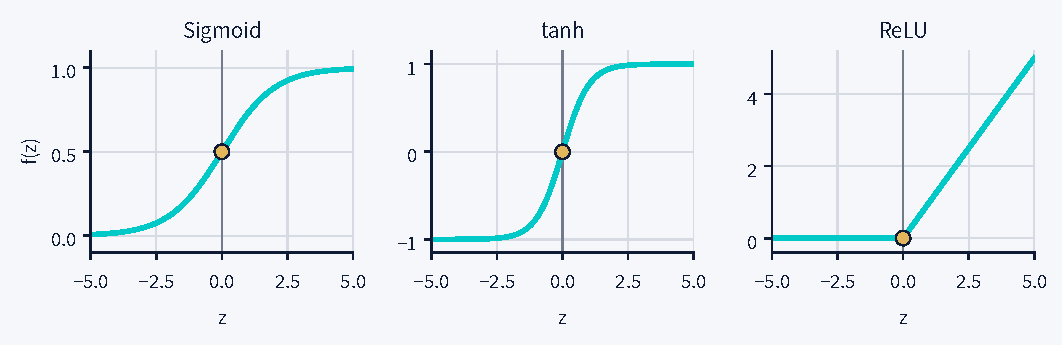
\includegraphics[width=\linewidth]{assets/charts/fig3_1_activations.pdf}
\caption{שלוש פונקציות הפעלה}\label{fig:3.1}
\figurenote{מקור: חישוב מהנוסחאות שב-\cite{S-ch03-01} (אין נתונים אמפיריים)}
\end{figure}
\begin{conceptbox}{פונקציית הפעלה}
פונקציית הפעלה (activation function) היא הכלל שקובע מה יוצא מנוירון בהינתן הסכום המשוקלל שלו. יש לה גם פרשנות ביולוגית: במודל של CS231n היא ממדלת את קצב הירי של הנוירון, כלומר באיזו תדירות הוא שולח אותות \cite{S-ch03-01}.
לאימון דרוש לה גם שיפוע מוגדר. אצל ReLU קבעו נאיר והינטון שהשיפוע הוא 0 כשהקלט קטן מאפס או שווה לו, ו-1 כשהוא חיובי, והתעלמו מהשבר שבנקודה 0 עצמה \cite{S-ch03-02}.
\end{conceptbox}
\section{משכבה לשכבה}
כבר נוירון אחד לבדו מסוגל לחזות. אם מפרשים את הפלט של נוירון עם סיגמואיד כהסתברות שדוגמה שייכת לאחת משתי קבוצות, ומאמנים אותו בהתאם, מתקבל מסווג בינארי, שמוכר גם בשם רגרסיה לוגיסטית (logistic regression) \cite{S-ch03-01}. כאן, לראשונה, מספרים הופכים לתחזית.
אבל הכוח האמיתי טמון בחיבור. ברשת נוירונים הנוירונים מסודרים בשכבות ומקושרים בגרף שאין בו מעגלים, כך שהמידע זורם קדימה ואינו חוזר אל עצמו \cite{S-ch03-01}. בשכבה מחוברת במלואה (fully-connected) כל נוירון מקושר לכל נוירון בשכבה הסמוכה, ואילו בין נוירונים באותה שכבה אין קשר בכלל \cite{S-ch03-01}. הפלט a של כל נוירון הופך לאחד הקלטים x של השכבה הבאה. השכבות שבין הקלט לפלט נקראות שכבות חבויות (hidden layers), ולשכבת הפלט בדרך כלל אין פונקציית הפעלה \cite{S-ch03-01}. ובספירה יש מוסכמה: כשאומרים "רשת בת N שכבות", לא סופרים את שכבת הקלט \cite{S-ch03-01}.
כמה פרמטרים יש בלוח כזה? חומרי הקורס עורכים חשבון: ברשת עם שלושה קלטים, שכבה חבויה של ארבעה נוירונים ושכבת פלט של שניים, יש 20 משקולות (3$\times$4 ועוד 4$\times$2) ו-6 הטיות, אחת לכל נוירון, ובסך הכול 26 פרמטרים נלמדים. מוסיפים שכבה חבויה שנייה של ארבעה ומצמצמים את הפלט לנוירון יחיד, וכבר יש 32 משקולות (3$\times$4, ועוד 4$\times$4, ועוד 4$\times$1) ו-9 הטיות, כלומר 41 \cite{S-ch03-01}. רשת זעירה, עשרות משקולות. וכשמערימים שכבות רבות, כל שכבה בונה את התיאור שלה מתוך התיאור של קודמתה \cite{S-ch01-05}, ומספר הפרמטרים מטפס במהירות.
\begin{figure}[htbp]
\centering
% Figure 3.2: one neuron and a small 3-4-2 network (structure and parameter count after S-ch03-01).
\begin{bookdiagram}[x=1cm,y=1cm]
  \tikzset{io/.style={circle,draw=turquoise,line width=0.9pt,fill=white,minimum size=8mm,inner sep=0pt}}
  % single neuron, read left to right like the formula
  \node[io] (x1) at (0,1.6) {$x_1$};
  \node[io] (x2) at (0,0.6) {$x_2$};
  \node at (0,-0.25) {$\vdots$};
  \node[io] (xn) at (0,-1.2) {$x_n$};
  \node[circle,draw=midnight,line width=1.2pt,fill=white,minimum size=11mm,font=\Large] (sum) at (4,0.2) {$\Sigma$};
  \draw[flow] (x1) -- node[above,sloped,font=\footnotesize] {$w_1$} (sum);
  \draw[flow] (x2) -- node[above,sloped,font=\footnotesize] {$w_2$} (sum);
  \draw[flow] (xn) -- node[below,sloped,font=\footnotesize] {$w_n$} (sum);
  \node[draw=gold,line width=1pt,rounded corners=1mm,fill=white,inner sep=1.5mm] (b) at (4,2.0) {הטיה $b$};
  \draw[flow] (b) -- (sum);
  \node[blk,minimum width=13mm,minimum height=10mm] (f) at (6.6,0.2) {$f$};
  \draw[flow] (sum) -- node[above] {$z$} (f);
  \node[io] (a) at (9,0.2) {$a$};
  \draw[flow] (f) -- (a);
  \node[font=\footnotesize,anchor=north] at (6.6,-0.5) {פונקציית הפעלה};
  \node[font=\footnotesize,anchor=north] at (9,-0.5) {פלט};
  \node[font=\footnotesize,anchor=north] at (0,-1.75) {קלטים};
  % small network 3 -> 4 -> 2
  \begin{scope}[yshift=-5.4cm]
    \foreach \j in {1,2,3}{\node[circle,draw=turquoise,line width=0.9pt,fill=white,minimum size=6.5mm] (i\j) at (1.5,{1.15-0.9*(\j-1)}) {};}
    \foreach \j in {1,2,3,4}{\node[circle,draw=violet,line width=0.9pt,fill=violet!22,minimum size=6.5mm] (h\j) at (4.2,{1.6-0.9*(\j-1)}) {};}
    \foreach \j in {1,2}{\node[circle,draw=turquoise,line width=0.9pt,fill=white,minimum size=6.5mm] (o\j) at (6.9,{0.7-0.9*(\j-1)}) {};}
    \foreach \p in {1,2,3}{\foreach \q in {1,2,3,4}{\draw[turquoise,line width=0.6pt] (i\p) -- (h\q);}}
    \foreach \p in {1,2,3,4}{\foreach \q in {1,2}{\draw[turquoise,line width=0.6pt] (h\p) -- (o\q);}}
    \node[font=\footnotesize] at (1.5,-1.75) {שכבת קלט};
    \node[font=\footnotesize] at (4.2,-1.75) {שכבה חבויה};
    \node[font=\footnotesize] at (6.9,-1.75) {שכבת פלט};
    \node[draw=gold,line width=1.2pt,rounded corners=1.5mm,fill=white,inner sep=2mm,align=center,font=\headingfont] at (10.0,0.25)
      {20 משקולות + 6 הטיות\\= 26 פרמטרים};
  \end{scope}
\end{bookdiagram}

\caption{נוירון אחד ורשת קטנה}\label{fig:3.2}
\figurenote{מקור: מסגרת הספר; מבנה הרשת וספירת הפרמטרים לפי \cite{S-ch03-01}}
\end{figure}
\section{מה נשאר מהמוח}
השם "נוירון" לא נבחר במקרה, ורשימות הקורס של סטנפורד אכן מקדישות סעיף להשראה הביולוגית. הנוירון הוא יחידת החישוב הבסיסית של המוח: הוא קולט אותות דרך הדנדריטים ושולח אות דרך אקסון יחיד, והמשקולות מקבילות לעוצמת הסינפסות \cite{S-ch03-01}. הערכה שמצוטטת שם מדברת על כ-86 מיליארד נוירונים במערכת העצבים של האדם, המחוברים בכ-10\textasciicircum{}14 עד 10\textasciicircum{}15 סינפסות \cite{S-ch03-01}.
גם כמה ציוני דרך מוקדמים בתולדות התחום נושאים את הזיקה למוח כבר בכותרתם. ב-1943 פרסמו מקאלוק ופיטס (Warren S. McCulloch, Walter Pitts) מאמר ששמו מדבר על "פעילות עצבית": "A logical calculus of the ideas immanent in nervous activity" \cite{S-ch03-04}. ב-1958 פרסם פרנק רוזנבלט ב-Psychological Review את "The perceptron", שכותרתו מציגה אותו כמודל הסתברותי לאחסון ולארגון של מידע במוח \cite{S-ch03-03}.
אבל אותו מדריך ממהר גם להזהיר: המודל הזה של נוירון ביולוגי גס מאוד \cite{S-ch03-01}.
\begin{mythbox}
\mythlabel רשת נוירונים היא מוח דיגיטלי קטן, והנוירונים שלה פועלים כמו אלה שבראשנו.
\tcblower
\realitylabel צוות הקורס בסטנפורד מונה ארבעה פערים לפחות \cite{S-ch03-01}. במוח יש סוגים רבים של נוירונים, שונים זה מזה בתכונותיהם. הדנדריטים לבדם מבצעים חישובים לא-ליניאריים מורכבים. סינפסה אינה מספר יחיד, אלא מערכת דינמית מסובכת. ובמערכות רבות התזמון המדויק של כל פולס חשמלי חשוב, בעוד שהמודל המלאכותי מסתפק בקצב. המדריך אף מציע להסביר רשתות נוירונים בלי שום השוואה למוח, ומזהיר שמי שיש לו רקע במדעי המוח עלול להיאנח למשמע השוואות כאלה \cite{S-ch03-01}.
\end{mythbox}
הנוירון של הספר הוא אפוא קריקטורה מתמטית מוצלחת: ההשראה שאולה מהביולוגיה, אבל הנאמנות שמורה לחשבון.
\section{בחזרה אל השאלה}
עכשיו אפשר לשוב אל הקוראת. היא עדיין עומדת ליד השיש ומביטה במסך, ואינה רואה דבר ממה שמתרחש מאחוריו. השאלה שלה, שהומרה למספרים, עוברת שכבה אחר שכבה. בכל נוירון אותו טקס קטן: מכפלות, סכום, הטיה, ברז. אף שלב בדרך לא יודע שמדובר בבצק, ואף משקולת לא "מבינה" מה היא שוקלת. ובכל זאת, בקצה השני של המערכת מתחילות להופיע מילים, אחת אחרי השנייה.
איך מודל שפה שלם הופך את זרם המספרים הזה לתשובה, מילה אחר מילה? לשם נמשיך בפרק 4.
\begin{insightsbox}
\begin{itemize}
\item נוירון מלאכותי עושה שלושה דברים פשוטים: מכפיל קלטים במשקולות, מוסיף הטיה ומעביר את הסכום דרך פונקציה לא-ליניארית \cite{S-ch03-01}.
\item המשקולות וההטיות הן הכפתורים שהאימון מכוונן \cite{S-ch03-01,S-ch01-05}. בתוך המכונה אין "בצק", יש רק מספרים כאלה.
\item פונקציית ההפעלה מכריעה כמה מהסכום עובר הלאה, והבחירה בה משפיעה על מהירות האימון ועל יציבותו \cite{S-ch03-01}.
\item השכבות הופכות יחידות זעירות למבנה שבונה תיאור על גבי תיאור, ומספר הפרמטרים גדל עם כל שכבה \cite{S-ch03-01,S-ch01-05}.
\item ההשראה ביולוגית, אבל הדמיון גס: רשת נוירונים היא מודל מתמטי, לא העתק של מוח \cite{S-ch03-01}.
\end{itemize}
\end{insightsbox}
